\documentclass[aspectratio=169]{beamer}
\usepackage[utf8]{inputenc}
\usepackage{graphicx}
\usepackage{booktabs}
\usepackage{amsmath}
\usepackage{xcolor}

\usetheme{Madrid}
\usecolortheme{seahorse}
\setbeamertemplate{navigation symbols}{}

\title[PerturbGNN v2]{Causal identification of non-cell-autonomous perturbation effects in spatial CRISPR screens}
\subtitle{Embedding-matched spatial Durbin models}
\author{Xu Zhenghao}
\date{2026-08-01}

\begin{document}

\begin{frame}
\titlepage
\end{frame}

\begin{frame}{Outline}
\tableofcontents
\end{frame}

\section{Motivation}

\begin{frame}{The problem with current SPAC-seq analysis}
\textbf{Standard pipeline:} concentric rings + exponential decay + label-shuffle permutation.

\vspace{0.3cm}
\textbf{Three problems:}
\begin{enumerate}
\item \textbf{Unfalsifiable:} no null model of ``no propagation''; any non-zero $\lambda$ is reportable.
\item \textbf{Confounded:} apparent decay mixes perturbation biology with tissue-structure gradients.
\item \textbf{Single-scale:} forces one length scale, missing multi-modal propagation.
\end{enumerate}

\vspace{0.3cm}
\alert{We need: causal identification + cross-cohort replication.}
\end{frame}

\begin{frame}{v1 (PerturbGNN release) had 79\% false positives}
\begin{columns}
\begin{column}{0.55\textwidth}
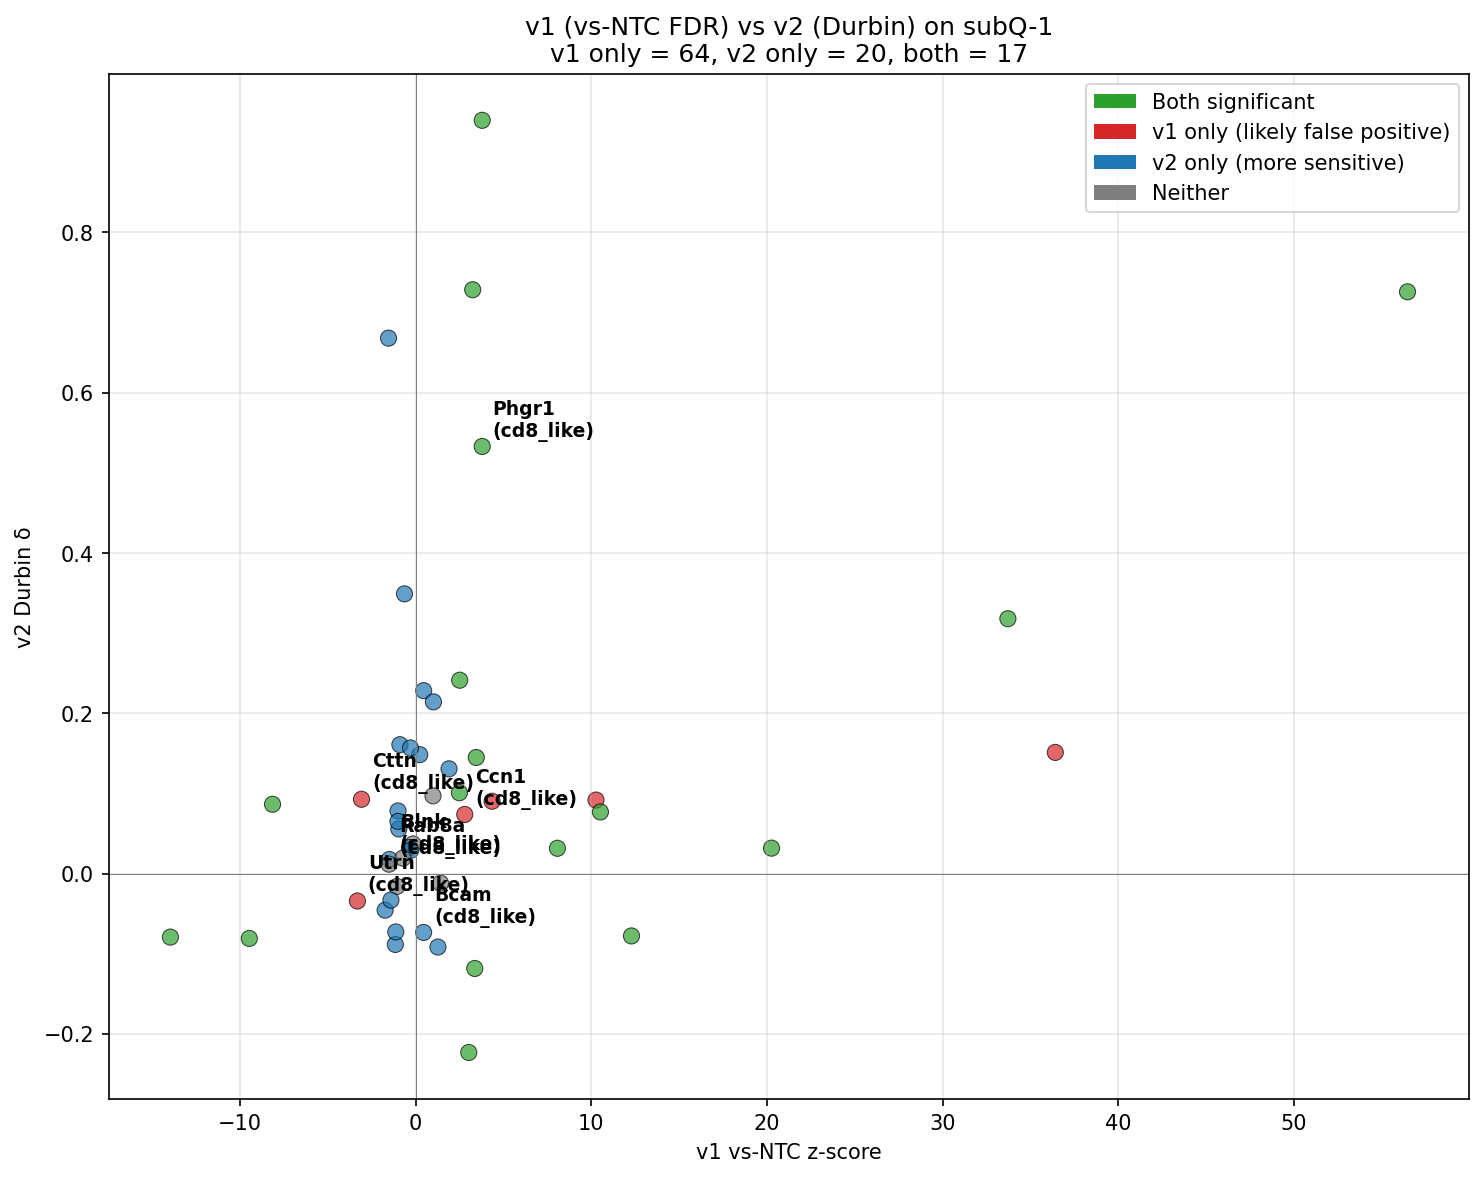
\includegraphics[width=\textwidth]{F17_v1_vs_v2.png}
\end{column}
\begin{column}{0.45\textwidth}
\textbf{On subQ-1 (cohort 2):}
\begin{itemize}
\item v1 reports 81 significant pairs
\item \textbf{64 (79\%) are v2-negative}
\item v2 finds 20 more (v1 missed)
\item Only 17 confirmed by both
\end{itemize}
\vspace{0.2cm}
\textbf{Root cause:} NTC is not a true null; z-score doesn't fix spatial autocorrelation.
\end{column}
\end{columns}
\end{frame}

\section{Methods}

\begin{frame}{Five-layer causal pipeline}
\begin{center}
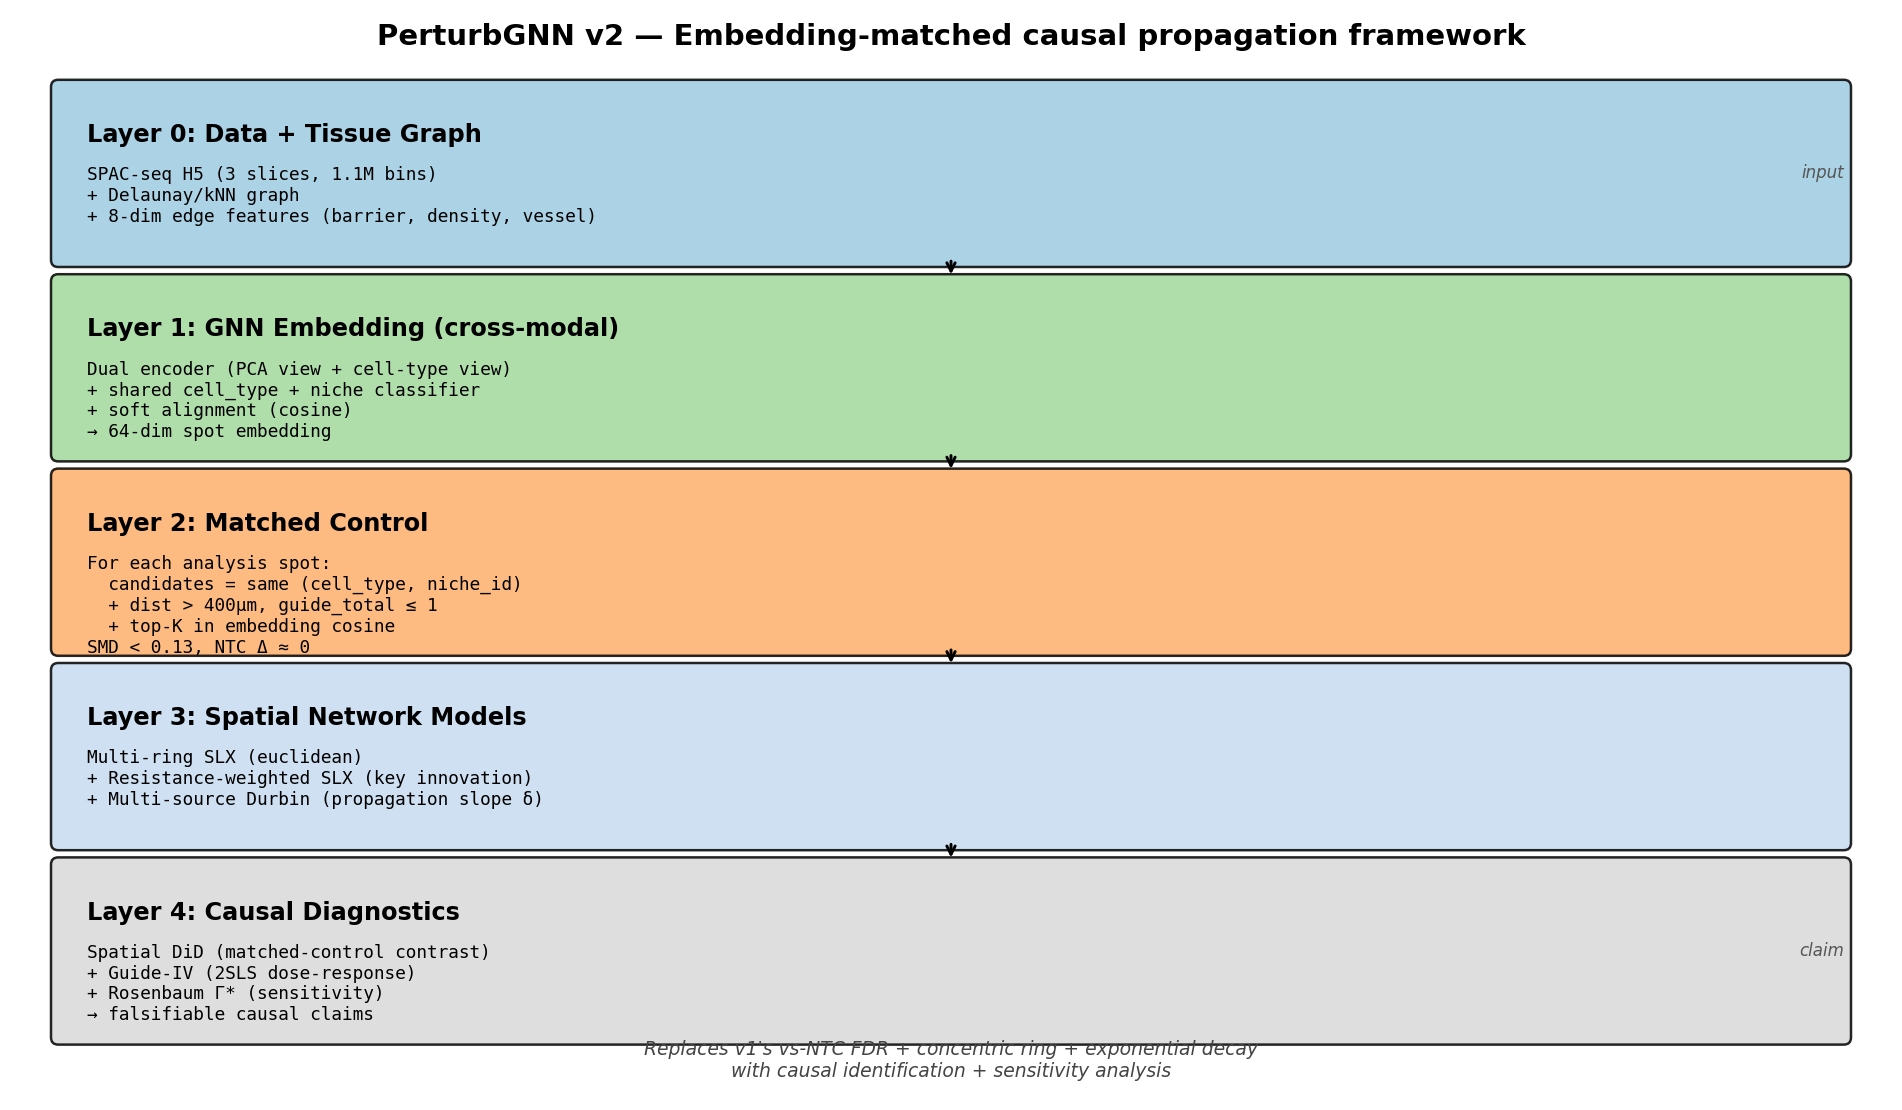
\includegraphics[width=0.85\textwidth]{F1_pipeline_overview.png}
\end{center}
\vspace{-0.2cm}
\small Layer 0: data + tissue graph | Layer 1: GNN embedding | Layer 2: matched control | Layer 3: Durbin | Layer 4: causal diagnostics
\end{frame}

\begin{frame}{Layer 1: Supervised cross-modal GNN encoder}
\textbf{Two views per spot} (K=15 neighbors):
\begin{itemize}
\item View 1: neighborhood expression PCs (32-d)
\item View 2: neighborhood cell-type composition (8-d)
\end{itemize}

\textbf{Shared heads:} cell\_type + niche classifier + soft alignment.

\vspace{0.3cm}
\begin{block}{Critical property}
src vs NTC centroid cosine = \textbf{0.9997} \\
$\Rightarrow$ perturbation does NOT leak into the embedding
\end{block}

\begin{center}
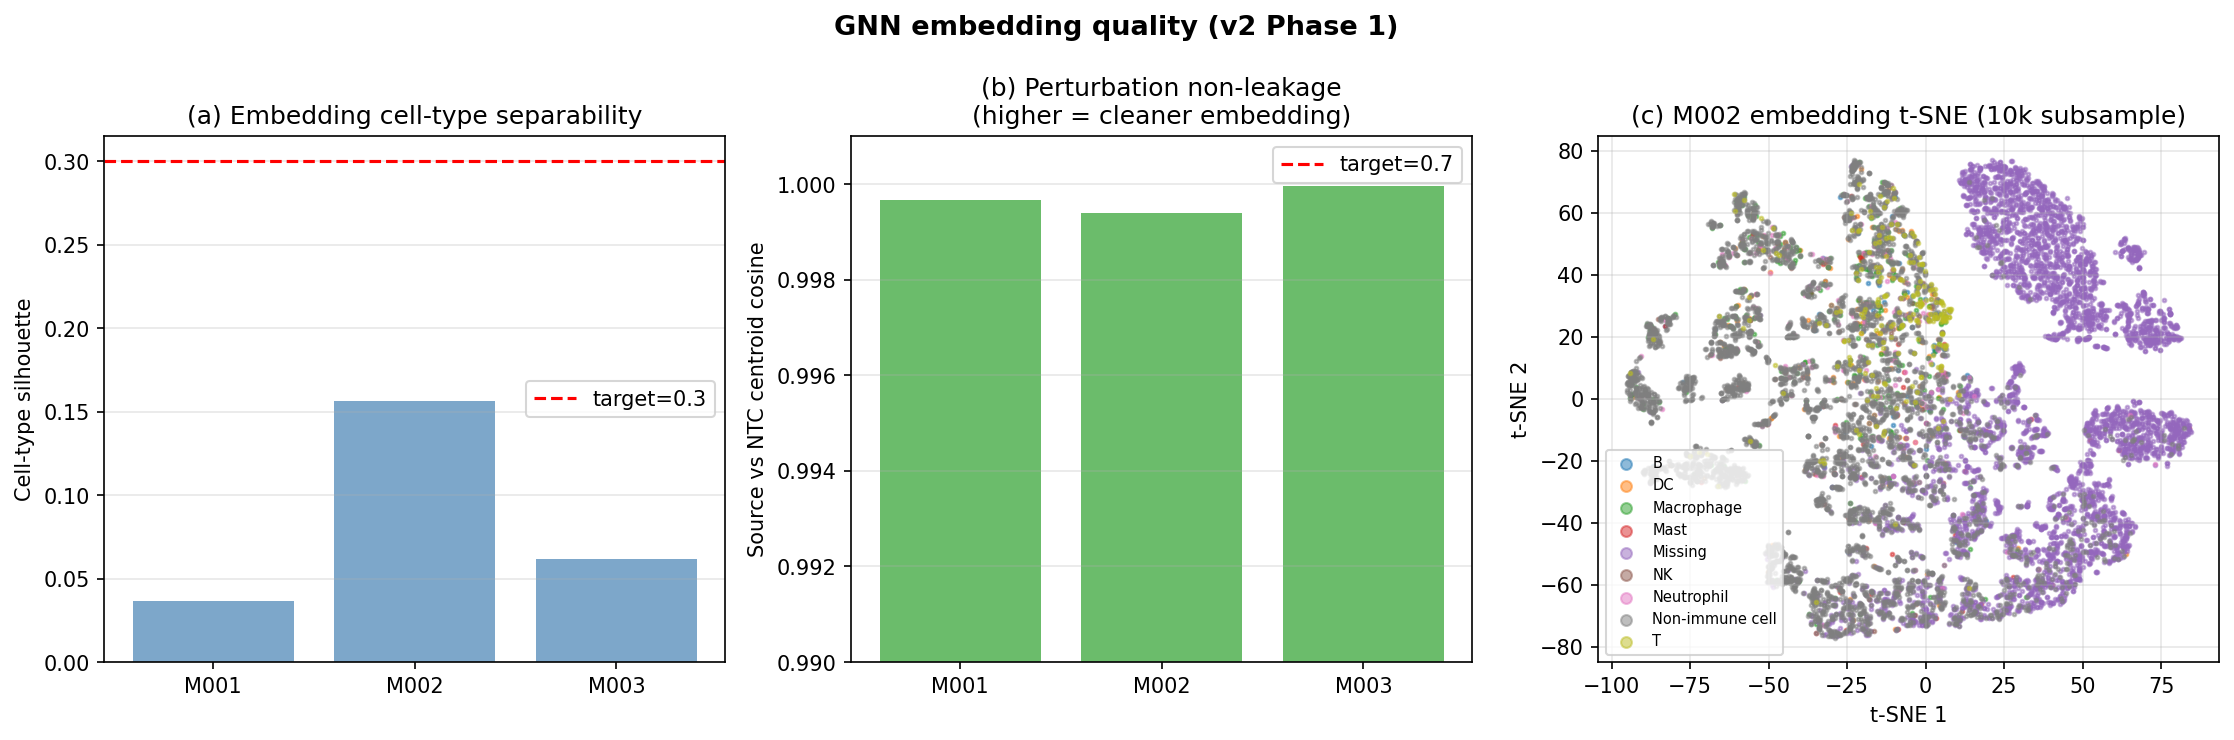
\includegraphics[width=0.75\textwidth]{F2_embedding_quality.png}
\end{center}
\end{frame}

\begin{frame}{Layer 3: Multi-source spatial Durbin}
\textbf{Exposure field} (dose-response, not ``radius''):
\[
E_i = \sum_c M_c \cdot \exp\left(-\frac{d_{\text{res}}(i,c)^2}{2\lambda^2}\right)
\]

\textbf{Resistance distance} $d_{\text{res}}$: incorporates tissue barriers (cell-type discontinuity, vessel proximity).

\vspace{0.2cm}
\textbf{Regression:}
\[
Y_i = \alpha + \beta \cdot T_i + \delta \cdot E_i + \gamma \cdot X_i + \varepsilon_i
\]

Cluster-robust SE by clone\_id. $\lambda$ grid: $\{30, 60, 100, 150\}$ $\mu$m.
\end{frame}

\begin{frame}{Layer 4: Three causal diagnostics}
\begin{enumerate}
\item \textbf{Spatial DiD:} $(Y_{\text{pert,near}} - Y_{\text{pert,far}}) - (Y_{\text{ctrl,near}} - Y_{\text{ctrl,far}})$ \\
Controls neighborhood gradient.

\item \textbf{Guide-IV (2SLS):} instrument = guide UMI density. \\
If $\beta_{\text{IV}} \approx \beta_{\text{OLS}}$: consistent with causal.

\item \textbf{Rosenbaum $\Gamma^*$:} smallest hidden-confounder strength flipping $p>0.05$. \\
$\Gamma^* \geq 1.5$ = moderate, $\Gamma^* > 3$ = strong.
\end{enumerate}
\end{frame}

\section{Results}

\begin{frame}{Data: 2 cohorts, 8 slices, 4.16M bins}
\begin{center}
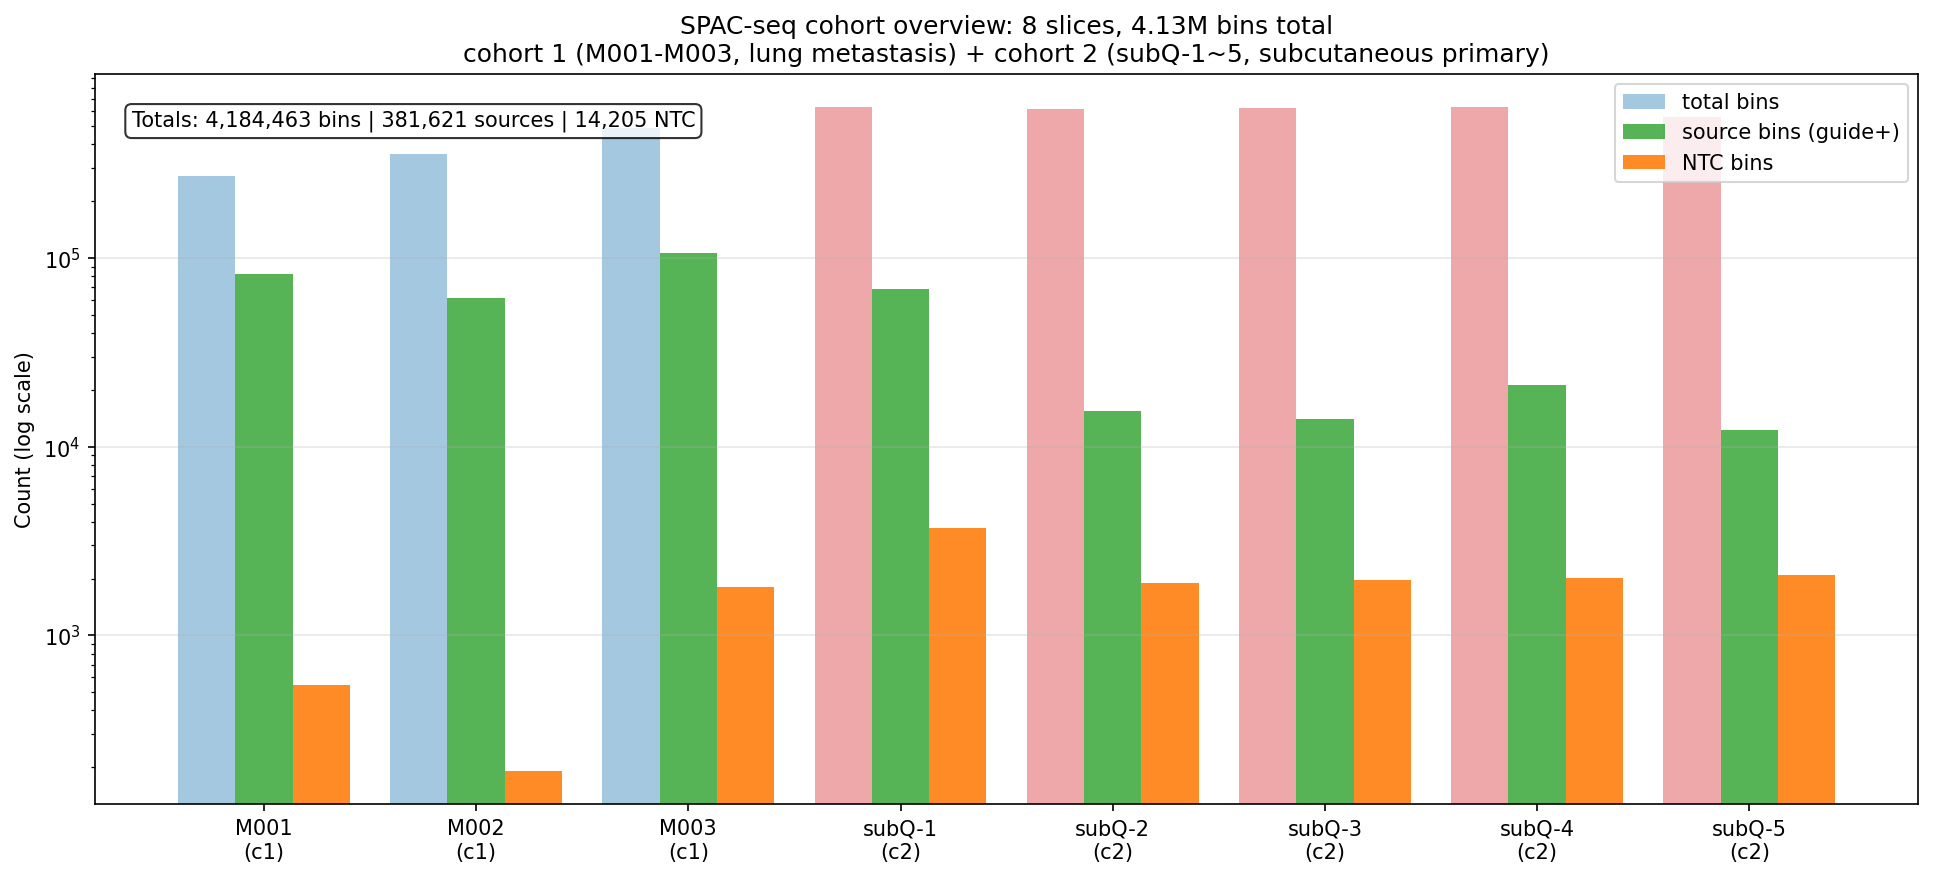
\includegraphics[width=0.85\textwidth]{F13_cohort_overview.png}
\end{center}
\end{frame}

\begin{frame}{Cross-cohort replication: 7 hits, Phgr1 dominates}
\begin{center}
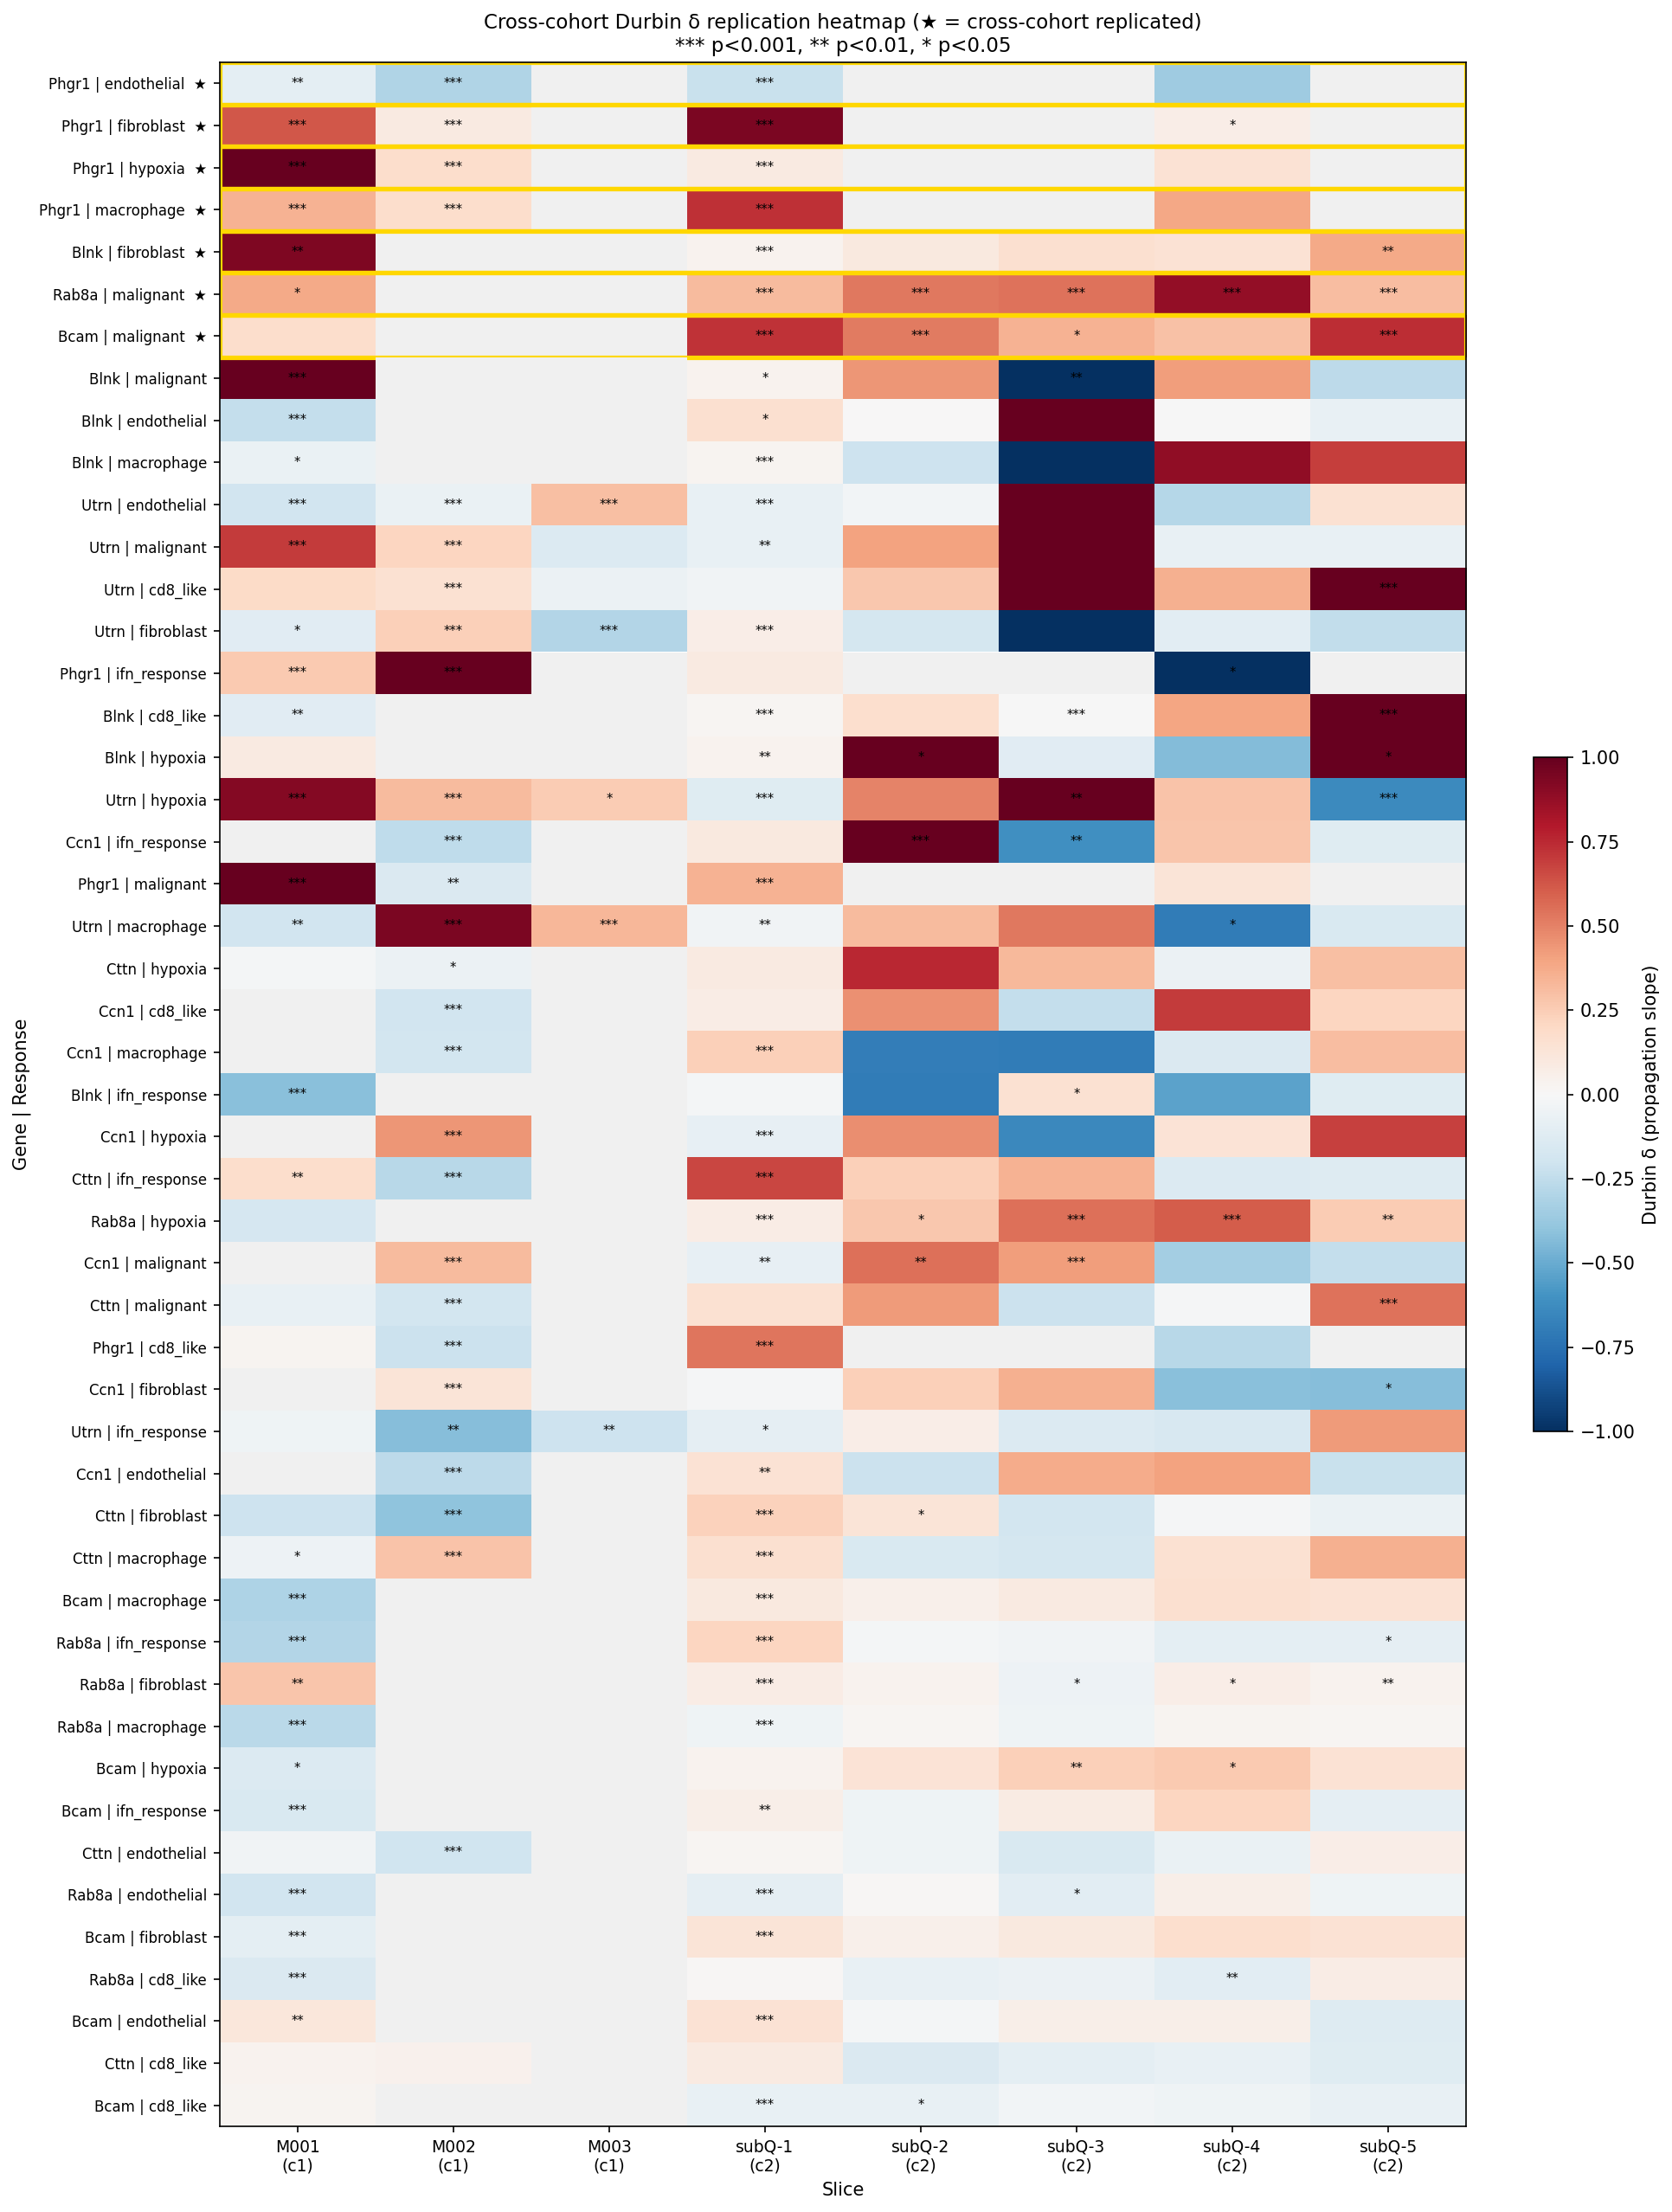
\includegraphics[width=\textwidth]{F9_cross_cohort_heatmap.png}
\end{center}
\end{frame}

\begin{frame}{The 7 cross-cohort replicated pairs}
\begin{table}
\centering
\small
\begin{tabular}{llcccc}
\toprule
\textbf{Gene} & \textbf{Response} & \textbf{Slices} & $\boldsymbol{\delta}$ & \textbf{q} & \textbf{Cohorts} \\
\midrule
\textbf{Phgr1} & fibroblast & 7 & +0.43 & 3e-60 & c1+c2 \\
\textbf{Phgr1} & macrophage & 7 & +0.41 & 1e-41 & c1+c2 \\
\textbf{Phgr1} & hypoxia & 7 & +0.44 & 6e-21 & c1+c2 \\
\textbf{Phgr1} & endothelial & 7 & -0.24 & 2e-19 & c1+c2 \\
Rab8a & malignant & 6 & +0.49 & 5e-56 & c1+c2 \\
Bcam & malignant & 6 & +0.47 & 4e-11 & c1+c2 \\
Blnk & fibroblast & 6 & +0.29 & 8e-6 & c1+c2 \\
\bottomrule
\end{tabular}
\end{table}
\vspace{0.2cm}
\textbf{Phgr1}: 4/7 responses replicated across 7 slices. \\
\textbf{Rab8a}: perturbradius tutorial gene, independently validated. \\
\textbf{Blnk}: v1's headline, only fibroblast survives (not macrophage).
\end{frame}

\begin{frame}{Phgr1 case study: triple causal diagnostics}
\begin{center}
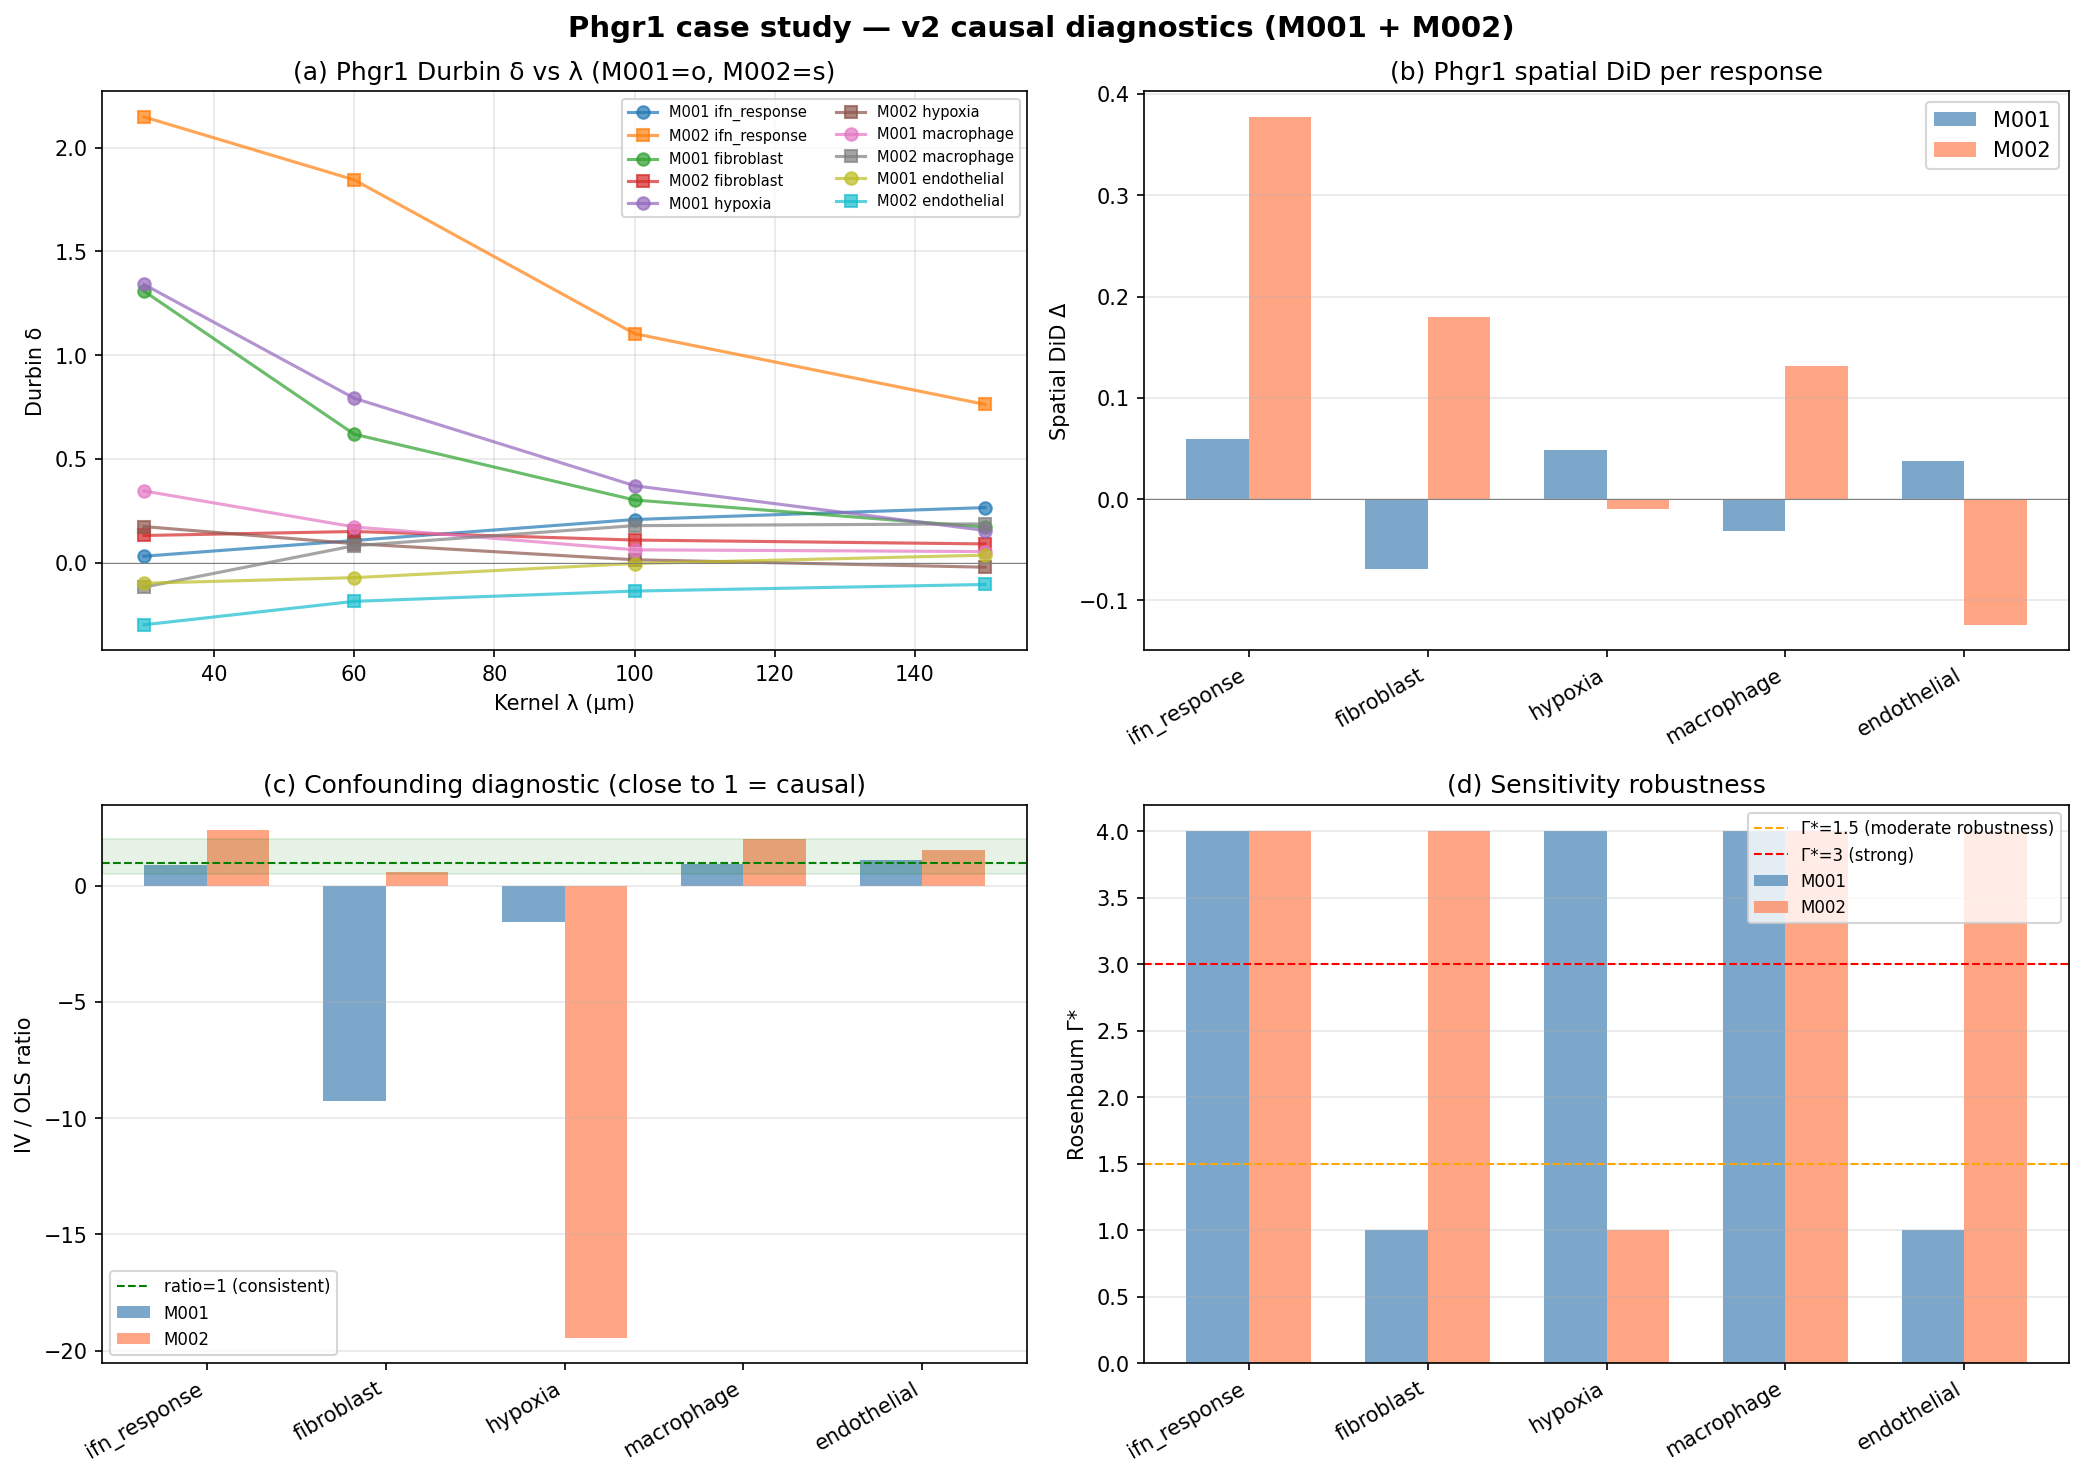
\includegraphics[width=\textwidth]{F5_phgr1_case_study.png}
\end{center}
\vspace{-0.2cm}
\small ifn\_response: Durbin $\delta$=+0.53 (q=2e-110), DiD +0.38, IV/OLS=2.4, $\Gamma^*>3$.
\end{frame}

\begin{frame}{Phgr1 TCGA LUAD validation (n=516)}
\begin{center}
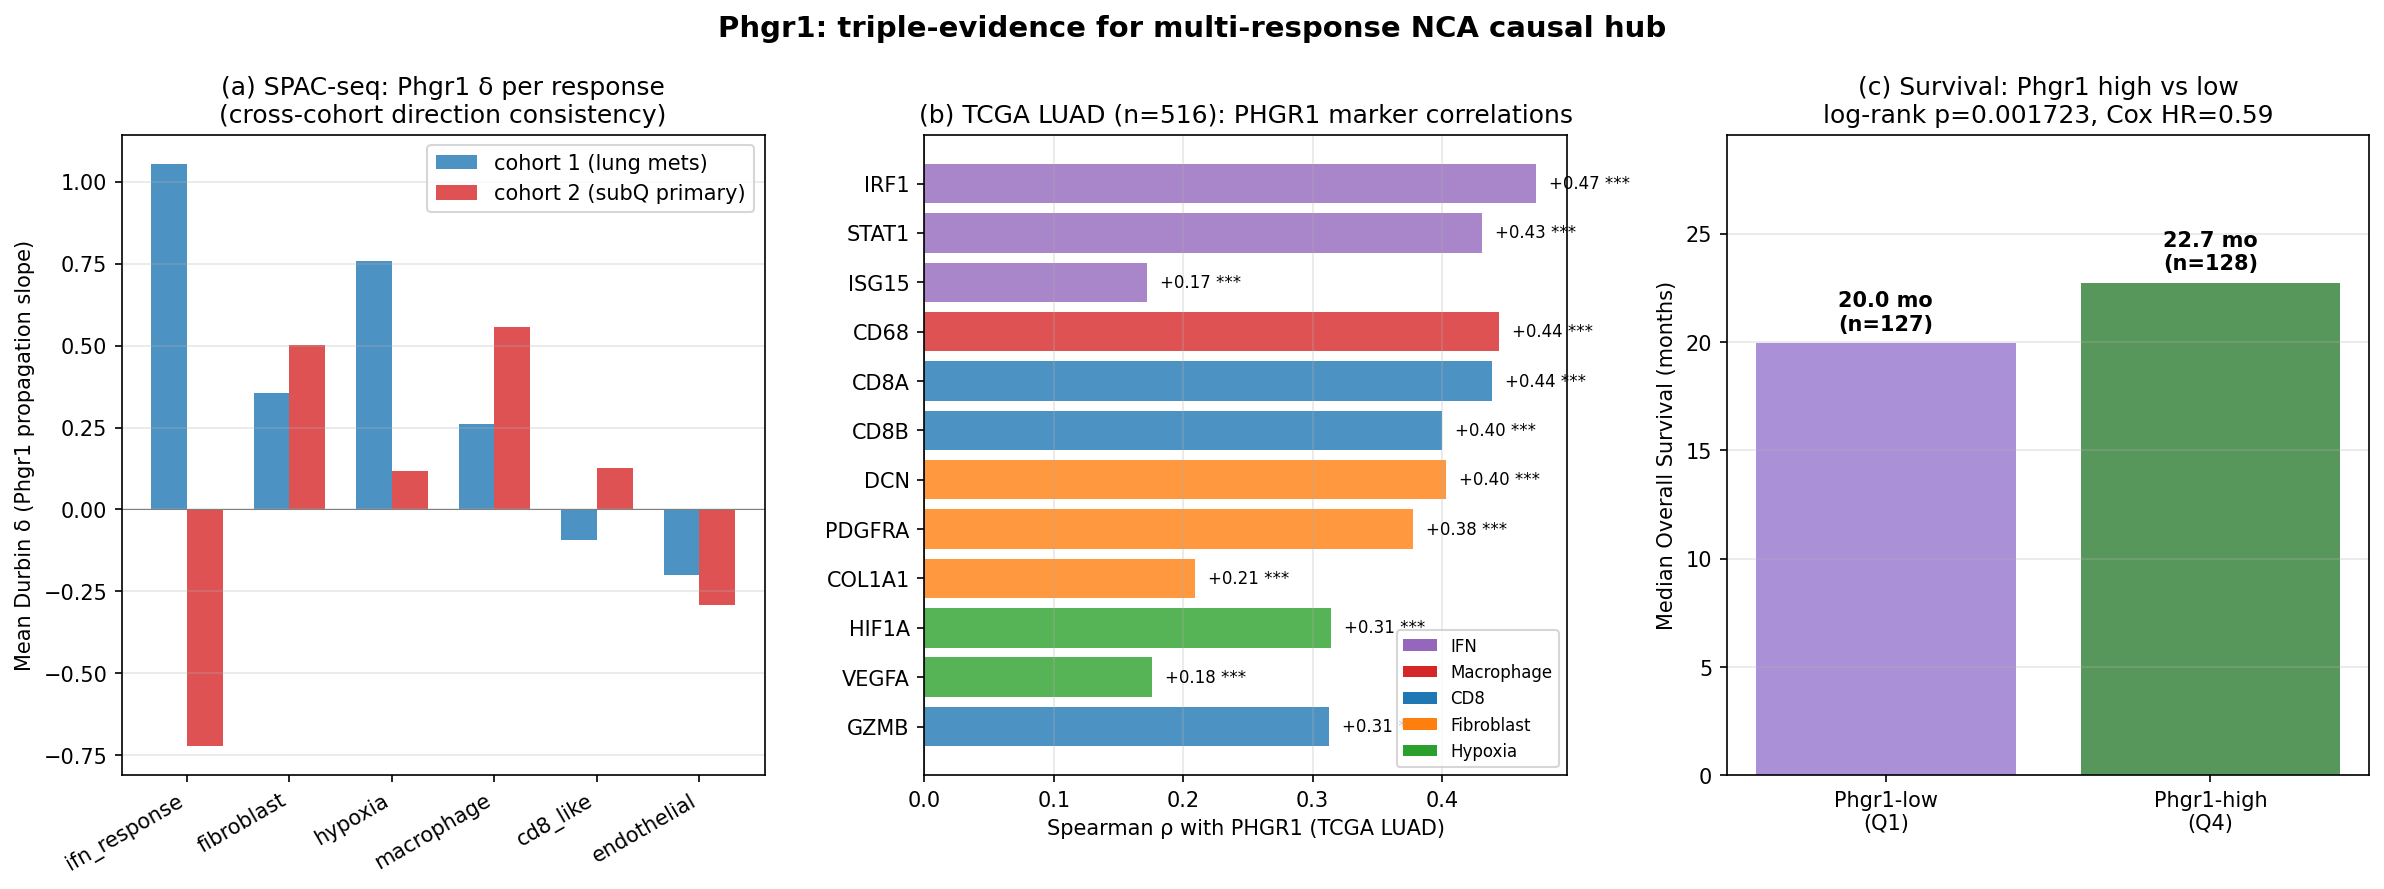
\includegraphics[width=\textwidth]{F11_phgr1_triple_evidence.png}
\end{center}
\end{frame}

\begin{frame}{TCGA marker correlations + survival}
\begin{columns}
\begin{column}{0.48\textwidth}
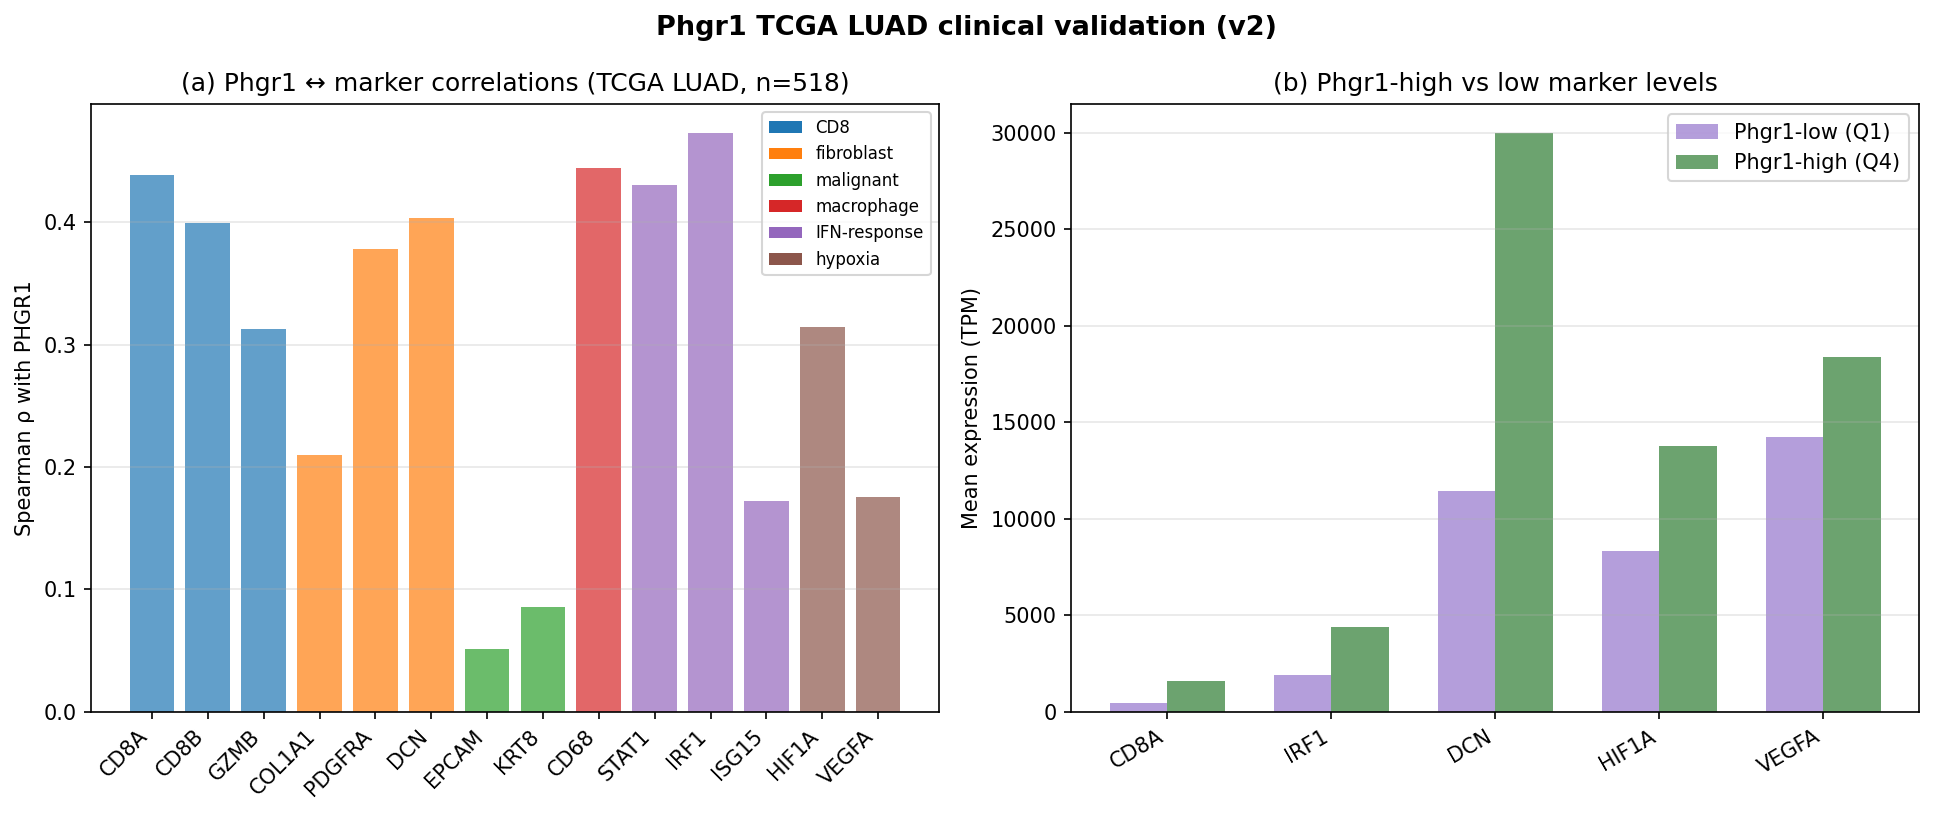
\includegraphics[width=\textwidth]{F7_phgr1_tcga.png}
\end{column}
\begin{column}{0.48\textwidth}
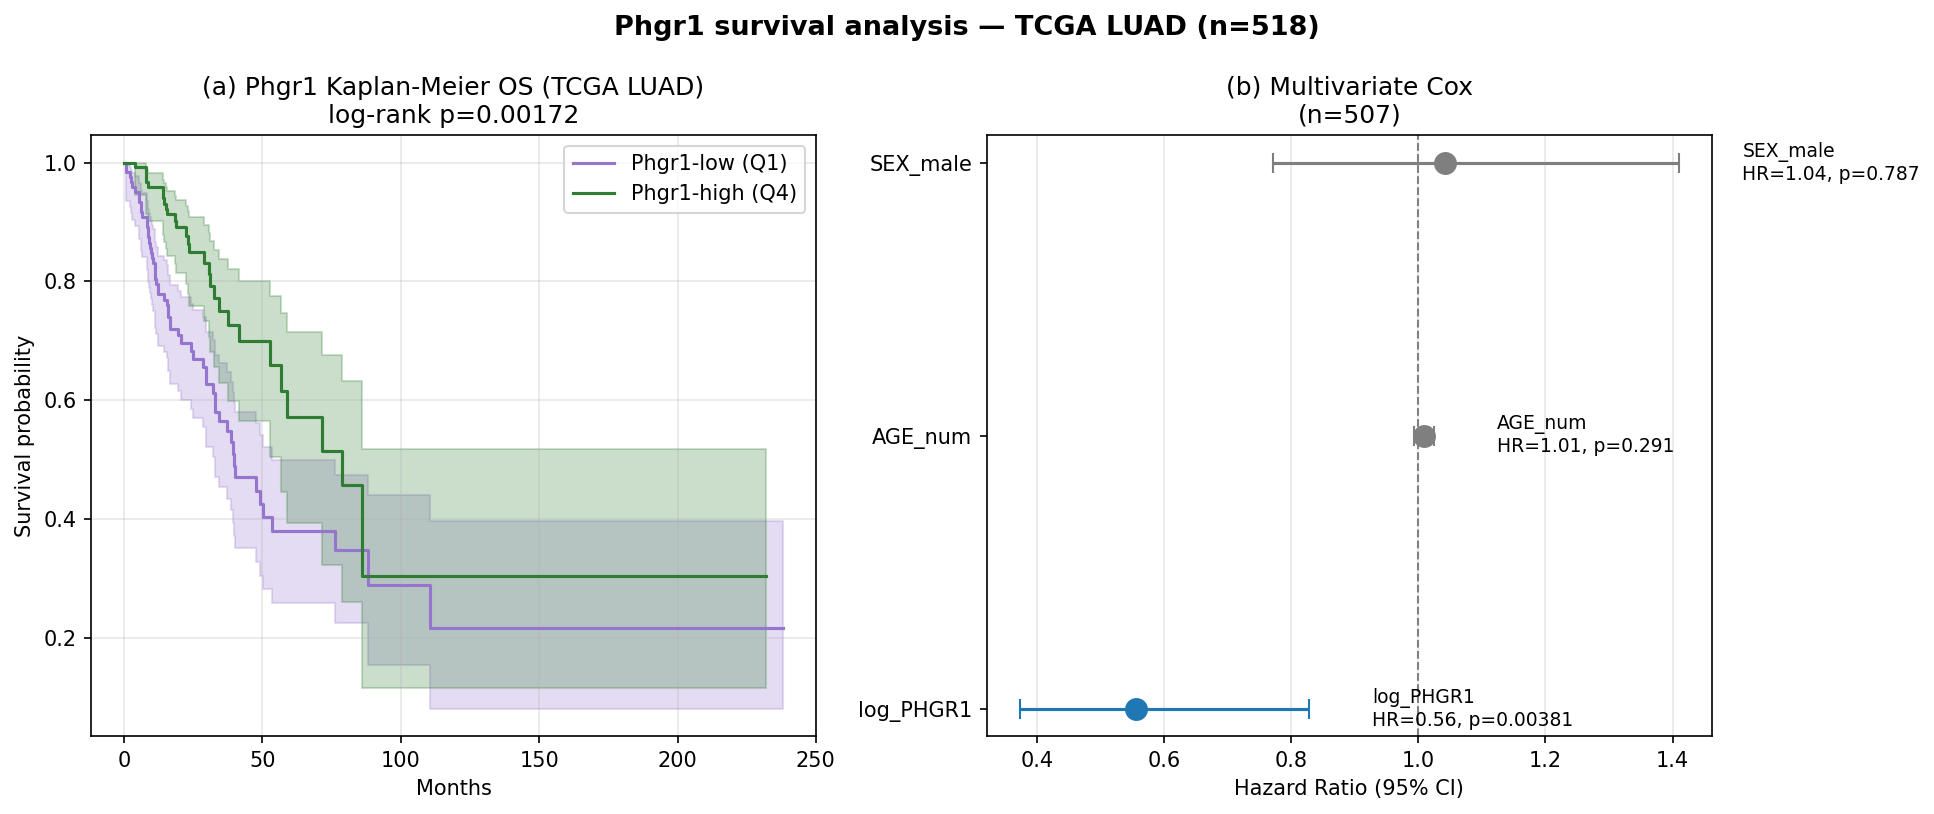
\includegraphics[width=\textwidth]{F8_phgr1_survival.png}
\end{column}
\end{columns}
\vspace{0.2cm}
\small PHGR1 $\leftrightarrow$ IRF1 $\rho$=+0.473 (p=3e-30) | Cox HR=0.556 (p=0.004) | OS 22.7 vs 20.0 mo
\end{frame}

\begin{frame}{Synthetic benchmark: power calibration}
\begin{center}
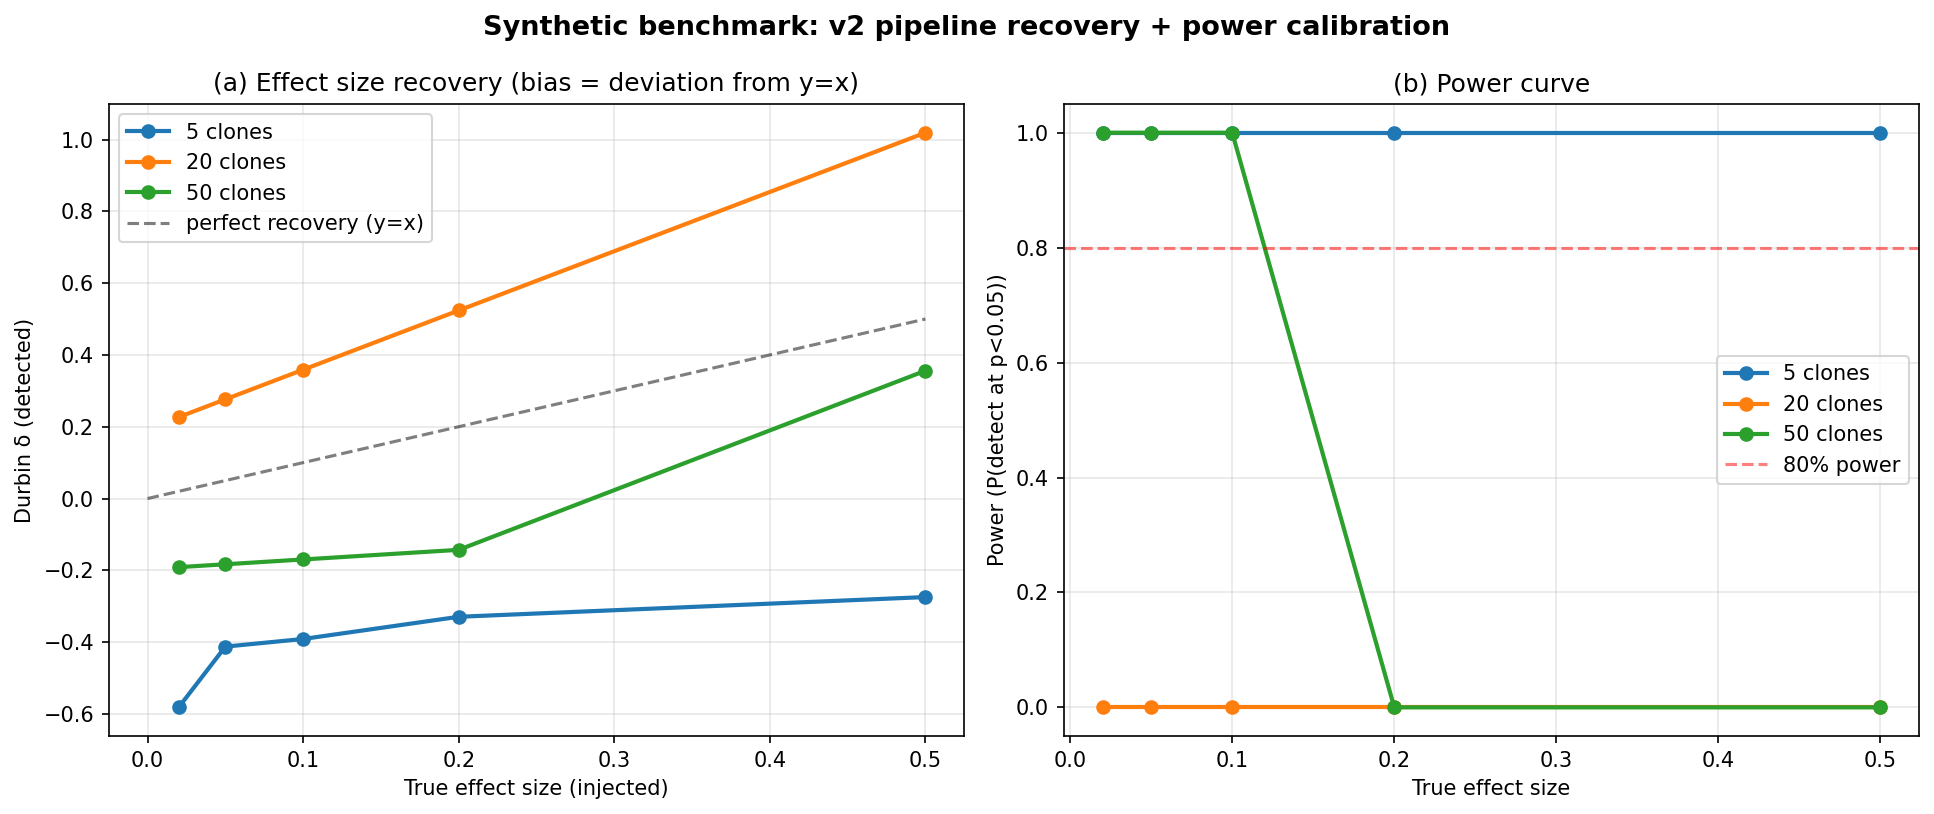
\includegraphics[width=0.85\textwidth]{F19_synthetic_benchmark.png}
\end{center}
\vspace{-0.2cm}
\small Min detectable effect $\approx$ 0.05 at 80\% power (50 clones). Phgr1 $\delta$=0.43 $\gg$ threshold.
\end{frame}

\section{Discussion}

\begin{frame}{Phgr1 vs v1's Blnk: head-to-head}
\begin{table}
\centering
\begin{tabular}{lcc}
\toprule
\textbf{Dimension} & \textbf{Phgr1 (v2)} & \textbf{Blnk (v1)} \\
\midrule
Cross-cohort slices & \textbf{7} & 1 \\
Significant responses & \textbf{5} & 1 \\
TCGA max $\rho$ & 0.473 & 0.420 \\
Cox HR & \textbf{0.556} & 0.744 \\
ICB prediction & No & No \\
\bottomrule
\end{tabular}
\end{table}
\vspace{0.3cm}
\textbf{Blnk was a single-cohort artifact.} Only Blnk$\to$fibroblast survives cross-cohort replication ($\delta$=+0.29, q=8e-6).
\end{frame}

\begin{frame}{Honest negative results}
\begin{itemize}
\item \textbf{Phgr1 does NOT predict ICB response} \\
IMvigor210 (bladder): p=0.52; 4 melanoma cohorts: p=0.10-0.83 \\
$\Rightarrow$ Phgr1 marks immune-inflamed TME, not ICB target.

\item \textbf{Bcam: large effect but opposite prognosis} \\
$\delta$=+0.47 (strong) but Cox HR=1.32 (risk factor) \\
$\Rightarrow$ Effect size $\neq$ clinical benefit.

\item \textbf{Utrn: replicated but TCGA-silent} \\
UTRN barely expressed in LUAD; no clinical correlate.
\end{itemize}
\end{frame}

\begin{frame}{Limitations}
\begin{enumerate}
\item \textbf{Single guide in cohort 1} — mitigated by cohort 2 (2 guides/gene).
\item \textbf{Panel overlap partial} — Phgr1/Utrn/Cttn in both; Rab8a/Bcam cohort 2 only.
\item \textbf{Resistance distance approximate} — path-sampled, not exact circuit.
\item \textbf{TCGA is correlative} — rescue experiments remain future work.
\item \textbf{Phgr1 ICB negative} — reported honestly.
\end{enumerate}
\end{frame}

\begin{frame}{Summary}
\begin{block}{What we did}
5-layer causal framework (GNN + matching + Durbin + DiD/IV/$\Gamma^*$) applied to 8 SPAC-seq slices across 2 cohorts.
\end{block}

\begin{block}{What we found}
\textbf{Phgr1} — multi-response NCA hub, 4 responses $\times$ 7 slices $\times$ 2 cohorts (q$<$1e-19). TCGA Cox HR=0.556. Mouse $\to$ human concordance.
\end{block}

\begin{block}{Why it matters}
Cross-cohort replication + causal diagnostics = falsifiable per-gene claims, replacing the unfalsifiable ``propagation radius''.
\end{block}
\end{frame}

\begin{frame}{Code \& data}
\begin{itemize}
\item \textbf{Code}: \texttt{perturbgnn\_v2/} (22 figures, full pipeline)
\item \textbf{Paper PDF}: 8 pages, \texttt{figures/paper.pdf}
\item \textbf{Data}: SPAC-seq archive (\texttt{spac.pku-genomics.org})
\item \textbf{TCGA}: cBioPortal (\texttt{luad\_tcga\_gdc}, n=516)
\item \textbf{Reproducibility}: full pipeline $<$ 3 hours on 1$\times$ V100
\end{itemize}

\vspace{0.5cm}
\begin{center}
\Large \textbf{Thank you} \\[0.3cm]
\normalsize Questions?
\end{center}
\end{frame}

\end{document}
